%% This is file `sample-sigconf.tex',
%% generated with the docstrip utility.
%%
%%
%% Commands for TeXCount
%TC:macro \cite [option:text,text]
%TC:macro \citep [option:text,text]
%TC:macro \citet [option:text,text]
%TC:envir table 0 1
%TC:envir table* 0 1
%TC:envir tabular [ignore] word
%TC:envir displaymath 0 word
%TC:envir math 0 word
%TC:envir comment 0 0
%%
\documentclass[sigconf,review,anonymous]{acmart}
%%
\AtBeginDocument{%
  \providecommand\BibTeX{{%
    Bib\TeX}}}

% Standard package includes
\usepackage{xcolor}
\usepackage[normalem]{ulem}
\usepackage{mathptmx}
\usepackage[T1]{fontenc}
\usepackage[utf8]{inputenc}
\usepackage{microtype}
\usepackage{graphicx}
\usepackage{listings}
\lstset{
  basicstyle=\small\ttfamily,
  breaklines=true,
  breakatwhitespace=false,
  frame=single,
  columns=fullflexible,
  keepspaces=true,
}
\usepackage{booktabs}
\usepackage{multirow}
\usepackage{amsmath}

\usepackage{enumitem}

\begin{document}

\title[Does the RAG Agent Know It Doesn't Know?]{Does the RAG Agent Know It Doesn't Know? Evaluating Uncertainty Awareness in Retrieval-Augmented Generation}

\author{Marta Sumyk}
\email{sumyk.pn@ucu.edu.ua}
\affiliation{%
  \institution{Ukrainian Catholic University}
  \city{Lviv}
  \country{Ukraine}
}

\author{Oleksandr Kosovan}
\email{o.kosovan@ucu.edu.ua}
\affiliation{%
  \institution{Ukrainian Catholic University}
  \city{Lviv}
  \country{Ukraine}
}

\author{Mykola Trokhymovych}
\email{mykola.trokhymovych@upf.edu}
\affiliation{%
  \institution{Pompeu Fabra University}
  \city{Barcelona}
  \country{Spain}
}

\renewcommand{\shortauthors}{Sumyk et al.}

\begin{abstract}
Retrieval-Augmented Generation (RAG) is widely used as a core component in autonomous agent systems. 
They answer questions by relying on retrieved passages. 
A critical failure happens when retrieval component returns topically-relevant but answer-free passages (a.k.a., hard negatives). 
We build a controlled benchmark from MIRACL hard-negative passages, split into three difficulty tiers based on TF-IDF similarity between the distractor and the gold passage. 
We evaluate four frontier models (GPT-5, GPT-4.1, Claude~Sonnet~4, Gemini~3.1~Flash~Lite) under two prompt conditions. 
We use GPT-5 as an LLM judge with a four-class taxonomy: ABSTAIN, HALLUCINATE, HEDGE, and CORRECT. 
As a result, we find three consistent patterns: (i) hallucination increases with distractor difficulty; (ii) models almost never hedge---they either abstain or hallucinate, with no middle ground; and (iii) an explicit abstention instruction reduces hallucination but leaves 12--22\% residual rates on hard distractors. 
These results show that Information Retrieval (IR) grounded uncertainty evaluation is essential for safe RAG deployment.
\end{abstract}

% \begin{CCSXML}
% <ccs2012>
%    <concept>
%        <concept_id>10002951.10003317.10003347.10003350</concept_id>
%        <concept_desc>Information systems~Question answering</concept_desc>
%        <concept_significance>500</concept_significance>
%    </concept>
%    <concept>
%        <concept_id>10010147.10010178.10010179</concept_id>
%        <concept_desc>Computing methodologies~Natural language generation</concept_desc>
%        <concept_significance>300</concept_significance>
%    </concept>
% </ccs2012>
% \end{CCSXML}

% \ccsdesc[500]{Information systems~Question answering}
% \ccsdesc[300]{Computing methodologies~Natural language generation}

\keywords{retrieval-augmented generation, hallucination, llm uncertainty, evaluation benchmark}

\maketitle

\section{Introduction}

Retrieval-Augmented Generation (RAG) has become a standard way to ground language model outputs in external knowledge~\cite{lewis2020rag}. 
The idea is simple: retrieve relevant passages, then generate an answer based on them. In agentic settings, this grounding is often the main trust mechanism~\cite{INSERT}.

However, this trust relies on a key assumption: that retrieval works. 
In practice, it often does not. Retrieval systems can return \textit{hard negatives}, passages that are topically related to a query but do not contain the answer~\cite{thakur2021beir,karpukhin2020dpr}. 
They discuss the right topic, use the right vocabulary, and pass relevance filters. They are, by design, the passages most likely to fool retrieval systems. 
When such a passage reaches a language model, the model faces a clear choice: recognize that the context is not useful and abstain, or go ahead and generate an answer.

In this study we want to understand: \textit{do RAG agents know when they don't know?} 
Specifically, we study what happens when a model receives a plausible but answer-free passage. 
We also ask whether this failure gets worse as the distractor becomes more deceptive.

We build our study based on IR benchmark, MIRACL dataset~\cite{zhang2023miracl}, which provides human-annotated positive passages and hard negatives retrieved by multiple systems.
The dataset allows us to stratify distractors by IR-grounded difficulty, measured as TF-IDF similarity to the gold passage.
It allows us to test whether the most IR-deceptive passages, are also the ones that cause the most hallucination. 
This connects our evaluation directly to the real-world RAG setting, where retrieval failures are not random noise but carefully selected hard negatives.

Across eight experiments with four frontier LLMs and two prompt conditions, we find three consistent patterns. 
First, hallucination rises with distractor difficulty. 
Second, models almost never hedge, they show a sharp binary pattern: abstain or hallucinate. 
Third, an explicit abstention instruction reduces hallucination but does not eliminate it.

% Prompt engineering alone cannot protect RAG deployments. 
% Retrieval quality directly drives hallucination risk. Measuring this failure is the first step to fixing it.

The main contributions of this work are:
\begin{itemize}[leftmargin=*]
  \item A controlled evaluation benchmark built from MIRACL hard negatives, stratified into three IR-grounded difficulty tiers;
  \item A multi-model empirical study showing consistent hallucination patterns and near-zero hedging across four frontier LLMs;
  \item Evidence that explicit abstention prompts provide partial but insufficient mitigation.
\end{itemize}


\section{Related Work}
In this section, we cover prior work on IR benchmarks, RAG evaluation, specifically for hallucination and uncertainty.

Standardised IR benchmarks such as BEIR~\cite{thakur2021beir} and MIRACL~\cite{zhang2023miracl} include hard-negative passages curated to challenge retrieval models. 
Dense retrieval training relies heavily on hard negatives~\cite{karpukhin2020dpr} to improve model discrimination. 
However, their downstream effect on RAG agent behavior has not been studied systematically.

Frameworks such as 
RAGAS~\cite{es2024ragas}, 
ARES~\cite{saadfalcon2024ares}, 
and RGB~\cite{chen2024benchmarking} 
evaluate RAG pipeline quality. They mostly focus on what happens when retrieval works, measuring faithfulness and relevance. 
They do not target what happens when retrieval returns misleading context.

Hallucination in LLMs has been extensively studied~\cite{ji2023survey}. 
In context-grounded generation, faithfulness (consistency with context) and factuality (consistency with world knowledge) are distinct properties~\cite{maynez2020faithfulness}. 
We apply this distinction to the RAG setting: we test whether models stay faithful to the signal that the context is insufficient.

LLM calibration and selective prediction have received growing attention~\cite{kadavath2022language}.
We complement this line of work by evaluating calibration specifically when context is a distractor.

\section{Benchmark Construction}

\subsection{Source Dataset}

We build our benchmark from the MIRACL Hard Negatives English split~\cite{10.1162/tacl_a_00595,enevoldsen2025mmtebmassivemultilingualtext,muennighoff2022mteb}. 
It provides 799 queries with human-annotated positive passages (containing the answer) and hard-negative passages retrieved by BM25, e5-multilingual-large, and e5-mistral-instruct. 
Using multiple retrievers ensures that the hard negatives are realistic failures from different production-grade systems. 
The full set contains 6,024 query-distractor pairs from 787 unique queries.

For each query, we use the first annotated positive as the \textit{gold passage}. 
This is only context given to the judge for evaluation, never to the answer generation model. 
All associated hard-negative passages serve as candidate distractors.

\subsection{Difficulty Stratification}

We quantify difficulty of the distractor passages as the TF-IDF cosine similarity with the gold passage. 
High similarity means the distractor is lexically and topically close to the correct source. We assume this makes it harder for the model to tell that the answer is missing. 
It is a natural consequence that a high-similarity distractor would rank near the top of retrieval results even for a strong system, because it looks like the answer passage without containing answer itself.

We compute similarity for all 6,024 pairs and split them into three equal parts: \textbf{Easy} ($<$0.10), \textbf{Medium} (0.10-0.22), and \textbf{Hard} ($>$0.22). 
From each tier, we select 100 examples, one per query, choosing the hardest available passage within the tier, resulting in a 300-sample stratified benchmark.

\subsection{Evaluation Protocol}

The full evaluation pipeline is shown in Figure~\ref{fig:pipeline}. 
Each sample contains a query and a distractor passage. 
The gold passage is never shown to the generation model. 
The model is prompted to answer using only the provided context. 
We adopt the LLM-as-judge approach~\cite{zheng2023judging} for response classification. 
In particular, we use GPT-5 as a judge, that prompted to evaluate the RAG output response against the gold passage using four labels:
\begin{itemize}
  \item \textbf{ABSTAIN}: the model declines to answer, citing insufficient context;
  \item \textbf{HALLUCINATE}: the model gives an answer not supported by or contradicted by the gold passage;
  \item \textbf{HEDGE}: the model expresses uncertainty (``possibly'', ``it seems'') but still attempts an answer;
  \item \textbf{CORRECT}: the model answers correctly (possible when a hard distractor shares partial information with the gold passage or the model has sufficient internal knowledge to answer the question).
\end{itemize}


\begin{figure}[t]
\centering
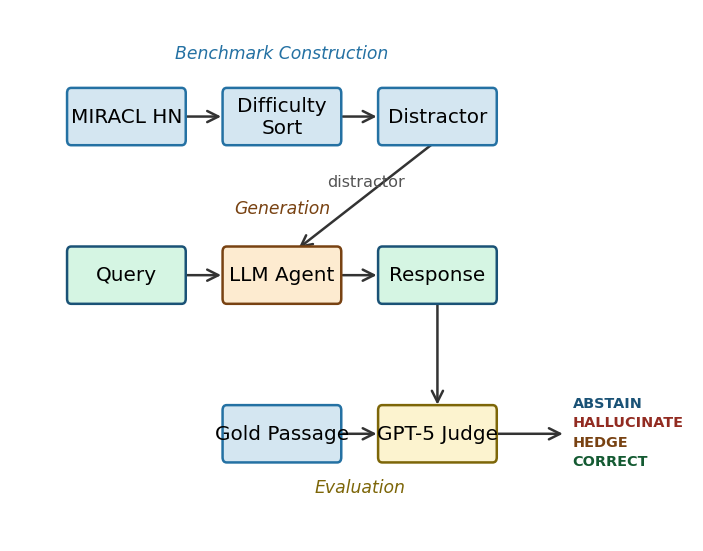
\includegraphics[width=\columnwidth]{figures/pipeline.png}
\caption{Evaluation pipeline schema.}
\label{fig:pipeline}
\end{figure}


\section{Experimental Setup}

In our experiments, we evaluate four frontier LLMs: GPT-5, GPT-4.1, Claude~Sonnet~4, and Gemini~3.1~Flash~Lite. 
All models are queried at temperature~0 for deterministic output.

We test two prompt variants:
\begin{itemize}
  \item \textit{Simple}: the model is instructed to use only the provided context and keep the answer concise.
  \item \textit{Advanced}: extends the simple prompt with an explicit abstention instruction: \textit{``If the context does not contain enough information to answer the question, explicitly state that you cannot answer based on the provided context.''}
\end{itemize}

This gives us 8 experiments (4 models $\times$ 2 prompt conditions), each evaluated on the fixed 300-sample benchmark.

\section{Results}

Table~\ref{tab:main_results} presents the full results. We report counts per class out of 100 for each difficulty tier. 
Figure~\ref{fig:hallucination} shows hallucination rates across difficulty levels for all conditions.

\begin{table}[t]
\centering
\caption{Results by model, prompt, and distractor difficulty. A\,=\,Abstain, H\,=\,Hallucinate, C\,=\,Correct. HEDGE $\leq$1\% across all conditions; omitted for brevity. Values are counts per 100 samples. P: S\,=\,Simple, Adv\,=\,Advanced.}
\label{tab:main_results}
\footnotesize
\setlength{\tabcolsep}{3.5pt}
\begin{tabular}{ll rrr rrr rrr}
\toprule
& & \multicolumn{3}{c}{\textbf{Easy}} & \multicolumn{3}{c}{\textbf{Medium}} & \multicolumn{3}{c}{\textbf{Hard}} \\
\cmidrule(lr){3-5}\cmidrule(lr){6-8}\cmidrule(lr){9-11}
\textbf{Model} & \textbf{P} & A & H & C & A & H & C & A & H & C \\
\midrule
\multirow{2}{*}{GPT-5}
  & S   & 70 & 27 & 3 & 66 & 26 &  8 & 50 & 33 & 17 \\
  & Adv & 81 & 17 & 2 & 76 & 18 &  6 & 65 & 18 & 17 \\
\midrule
\multirow{2}{*}{GPT-4.1}
  & S   & 72 & 21 & 7 & 71 & 18 & 11 & 53 & 29 & 18 \\
  & Adv & 84 & 13 & 3 & 81 & 10 &  9 & 64 & 22 & 13 \\
\midrule
\multirow{2}{*}{Cl.\ Son.\ 4}
  & S   & 81 & 15 & 4 & 75 & 21 &  4 & 59 & 32 &  8 \\
  & Adv & 88 & 11 & 1 & 86 & 10 &  4 & 71 & 21 &  8 \\
\midrule
\multirow{2}{*}{Gem.\ 3.1~FL}
  & S   & 78 & 20 & 2 & 83 & 11 &  6 & 60 & 21 & 19 \\
  & Adv & 92 &  7 & 1 & 89 &  6 &  5 & 74 & 12 & 14 \\
\bottomrule
\end{tabular}
\end{table}

\begin{figure}[t]
\centering
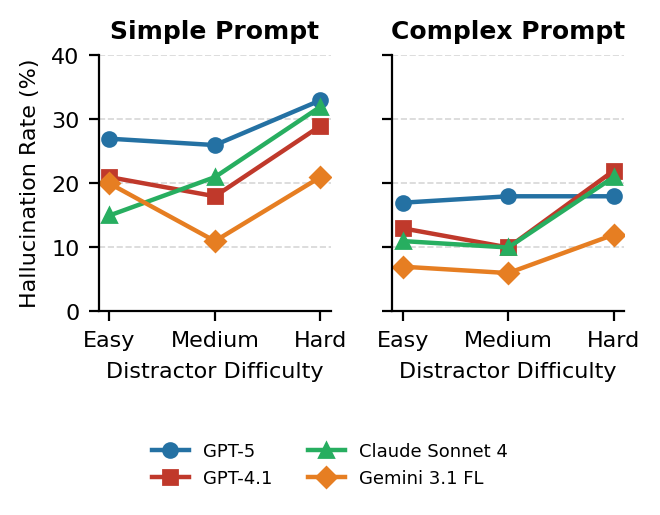
\includegraphics[width=\columnwidth]{figures/hallucination.png}
\caption{Hallucination rate (\%) by model and distractor difficulty. Simple prompt (left) vs.\ Advanced prompt (right).}
\label{fig:hallucination}
\end{figure}


Across all models and both prompt conditions, hallucination increases from Easy to Hard distractors in most cases. 
Under the simple prompt, GPT-5 rises from 27\% (Easy) to 33\% (Hard). Claude Sonnet~4 rises from 15\% to 32\%. 
This confirms that distractor difficulty is a reliable predictor of hallucination risk. 
The harder a distractor, the more likely the model is to treat it as sufficient evidence.

We also observe that the CORRECT rate rises with difficulty. 
This pattern reinforces our central finding: hard distractors causes the model to commit to an answer rather than abstain. 
When the model answers, it occasionally happens to be correct — but the driving force is overconfidence, not comprehension. 
The rising CORRECT rate is therefore further evidence of harder distractors weakening abstention behavior.

The HEDGE class appears at most once per experimental condition across all 8 experiments, giving rates $\leq$1\%. So, the models do not express partial uncertainty. 
Instead, they tend to either cleanly abstain or fully commit to a hallucinated response. 

Adding an explicit abstention instruction consistently reduces hallucination across all models (Figure~\ref{fig:hallucination}, right vs.\ left). 
The effect is strongest for easy distractors: Gemini's hallucination drops from 20\% to 7\%, and GPT-5's from 27\% to 17\%. 
However, the advanced prompt fails on hard distractors. Residual hallucination rates of 12--22\% remain: GPT-4.1 reaches 22\%, Claude Sonnet~4 reaches 21\%, GPT-5 reaches 18\%, and Gemini reaches 12\%. 
Even the most conservative model still hallucinates on roughly one in eight hard distractors under our experimental setup.
So, prompt engineering helps and costs almost nothing, but it cannot replace retrieval quality improvements or systematic evaluation.

Gemini~3.1~Flash~Lite achieves the lowest hallucination overall, especially under the advanced prompt (7\%/6\%/12\% across difficulty levels). 
GPT-4.1 and Claude~Sonnet~4 show broadly comparable mid-range behavior. This raises a potential self-consistency concern worth examining in future work.

\section{Discussion}

Hard negatives from standard retrieval pipelines are a real reliability risk. 
These passages are highly likely to be retrieved in production RAG systems, and they potentially can cause a significant amount of RAG errors.

The fact that hallucination persists even after adding an abstention instruction highlights retrieval component importance. 
This connects our findings to the broader IR research agenda: better retrieval is not only a ranking problem, it is a safety problem.

Our work also argues for IR-grounded uncertainty evaluation as a standard part of RAG benchmarking. 
Existing evaluation suites test whether models use correct context faithfully. 
Our benchmark design targets the complementary failure: what happens when retrieval returns misleading context? 
Because this failure persists even with the advanced prompting, measuring it is a prerequisite to improving it.

\paragraph{Limitations.}
Our evaluation is limited to English, 300 samples, and a single judge (GPT-5). 
Using GPT-5 as both a generation model and the judge introduces potential evaluation bias. 
Future work should include multilingual evaluation, larger sample sizes, alternative judges, and analysis of how retrieval quality improvements translate to uncertainty behavior.

\section{Conclusion}

To sum up, we presented a controlled benchmark design for evaluating uncertainty awareness in RAG under topically-deceptive retrieval failures. 
The benchmark is derived from MIRACL hard negatives and stratified by IR-grounded difficulty. 
Across eight experiments with four frontier LLMs, we showed three things: hallucination rises with distractor difficulty; models almost never hedge; and explicit abstention instructions reduce but do not eliminate hallucination---12--22\% residual rates persist on hard distractors. 
These findings show that retrieval quality and systematic IR-based uncertainty evaluation are both essential for reliable RAG deployment. 

\bibliographystyle{ACM-Reference-Format}
\bibliography{custom}

\end{document}